\section{Generative models}

\frame[<+->]{
	\frametitle{Why generative models?}
	Deep Learning
	\begin{itemize}
	\item[pro] Rich non-linear models for	classification and sequence prediction.
	\item[pro] Scalable learning using stochastic approximation and conceptually simple.
	\item[con] Only point estimates.
	\item[con] Hard to score models, do selection and complexity penalisation.
	\end{itemize}
	Probabilistic modelling
	\begin{itemize}
	\item[pro] Unified framework for model building, inference, prediction and decision making.
	\item[pro]  Explicit accounting for uncertainty and variability of predictions.
	\item[pro]  Robust to over-fitting.
	\item[pro]  Offers tools for model selection and composition.
	\item[con] Potentially intractable inference,
	\item[con] computationally expensive 
	\item[con] long simulation time.
	\end{itemize}
	
}

\frame[<+->]{
	\frametitle{Why generative models?}
\begin{itemize}

\item Lack of training data.
\item Partial supervision.
\item Lack of inductive bias.
\end{itemize}
	

}


\frame[<+->]{
	\frametitle{PGM}
	\begin{itemize}
	\item Inference in graphical models is the problem of computing a conditional probability distribution over the values of some of the nodes.
	\item We also want to compute marginal probabilities in graphical models, in particular the probability of the observed evidence.
	\item A latent variable model is a probabilistic model over observed and latent random variables.
	\item For a latent variable we do not have any observations.
	
	\end{itemize}
	
}


%\frame[<+->]{
%	\frametitle{}
	
	
%}




\section{Exact Marginal}

\frame{
	\frametitle{IBM 1-2}
	
	Latent alignment 
	\begin{itemize}
		\item Count-based models with EM is attempting to find the maximum-likelihood estimates for the data.
		\item Feature-rich Models (NN to combine features).
		\item Bayesian parametrisation of IBM. 
	\end{itemize}
	
}


\frame{
	\frametitle{IBM1: incomplete-data likelihood}
	
	\begin{columns}
	\begin{column}{0.2\textwidth}
	\begin{center}
    \scalebox{0.8}{
    \begin{tikzpicture}
    % Define nodes
    \node[obs]						(f)		{$ f $};
    \node[latent, above = of f]		(a)		{$ a $};
    \node[const, above = of a]		(m)		{$ m $};
    \node[obs, left = of f]		(e)		{$ e_0^{l} $};
    \node[const, above = of e]		(l)		{$ l $};
    
    % Connect nodes
    \edge{e,a}{f};
    \edge{l,m}{a};
    
    % add plates
    \plate {source-sentence} {(f)(a)} {$ m $};
    \plate {corpus} {(source-sentence) (e) (l) (m)} {$ S $};
    \end{tikzpicture}
    }
    \end{center}
    \end{column}
	\begin{column}{0.85\textwidth}
	
    Incomplete-data likelihood
    \begin{align}
    p(f_1^m|e_0^l) &= \sum_{a_1=0}^l \dotsb \sum_{a_m=0}^l p(f_1^m, a_1^m|e_{a_j}) \\
     &= \sum_{a_1=0}^l \dotsb \sum_{a_m=0}^l \prod_{j=1}^n p(a_j|l, m) p(f_j|e_{a_j}) \\
	 &= \prod_{j=1}^n \sum_{a_j=0}^l p(a_j|l, m) p(f_j|e_{a_j})
    \end{align}

	\end{column}	
	\end{columns}
	
    
}


\frame{
	\frametitle{IBM1: posterior}
		
	Posterior
	\begin{align}
	p(a_1^m|f_1^m, e_0^l) &= \frac{p(f_1^m, a_1^m|e_0^l)}{p(f_1^m|e_0^l)} 
	\end{align}
	
	Factorised
	\begin{align}\label{eq:paj}
		p(a_j|f_1^m, e_0^l) &= \frac{p(a_j|l, m) p(f_j|e_{a_j})}{\sum_{i=0}^l p(i|l, m) p(f_j|e_i)} 
	\end{align}
}


\frame{
\begin{adjustwidth}{-1.5em}{-1em}
	\frametitle{MLE via EM}
	
	E-step:
	\begin{small}
	\begin{align}
		\mathbb E[n(\mathsf e \rightarrow \mathsf f | a_1^m)] &= \sum_{a_1=0}^l \dotsb \sum_{a_m=0}^l p(a_1^m|f_1^m,e_0^l) n(\mathsf e \rightarrow \mathsf f | A_1^m)  \\
		&= \sum_{a_1=0}^l \dotsb \sum_{a_m=0}^l \prod_{j=1}^m p(a_j|f_1^m,e_0^l) \mathds 1_{\mathsf e}(e_{a_j}) \mathds 1_{\mathsf f}(f_j)  \\
		&= \prod_{j=1}^m \sum_{i=0}^l p(a_j = i|f_1^m,e_0^l) \mathds 1_{\mathsf e}(e_i) \mathds 1_{\mathsf f}(f_j) 
	\end{align}
	\end{small}
	
	M-step:
	\begin{align}
		\theta_{e, f} = \frac{\mathbb E[n(e \rightarrow f | a_1^m)]}{\sum_{ f'} \mathbb E[n( e \rightarrow  f' | a_1^m)]}
	\end{align}
\end{adjustwidth}
}


\frame{
	\frametitle{IBM 1-2: strong assumptions}
	
	Independence assumptions
	\begin{itemize}
		\item $p(a|m, n)$ does not depend on lexical choices\\
		a$_1$ \textcolor{red}{cute}$_2$ house$_3$ $\leftrightarrow$ una$_1$  casa$_3$  \textcolor{red}{bella}$_2$\\ \pause
		a$_1$ \textcolor{blue}{cosy}$_2$ house$_3$ $\leftrightarrow$ una$_1$ casa$_3$ \textcolor{blue}{confortable}$_2$ \\ \pause
		\item $p(f|e)$ can only reasonably explain one-to-one alignments\\		
		I \alert{will be leaving} \textcolor{blue}{soon} $\leftrightarrow$ \alert{voy a salir} \textcolor{blue}{pronto} \pause
	\end{itemize}
	
	~ 
	
	Parameterisation
	\begin{itemize}
		\item categorical events are unrelated \\
		prefixes/suffixes: normal, normally, abnormally, $\ldots$\\
		verb inflections: comer, comi, comia, comio, $\ldots$ \\
		gender/number: gato, gatos, gata, gatas, $\ldots$ 
		%\item number of parameters grows with data\\
		%$P(F|E)$ takes $O(v_F \times v_E)$ parameters
	\end{itemize}
	
}
\frame{
	\frametitle{\citet{Berg+2010:PU}}
	
	Lexical distribution in IBM model 1
	\begin{align}
		p(f|e) &= \frac{\exp(w_{\text{lex}}^\top h_{\text{lex}}(e, f))}{\sum_{f'} \exp(w_{\text{lex}}^\top h_{\text{lex}}(e, f'))} 
	\end{align}
	
	~
	
	Features
	\begin{itemize}
		\item $f \in V_F$ is a French word (decision), $e \in V_E$ is an English word (conditioning context), 
				$w \in R^d$ is the parameter vector, and $h : V_F \times V_E \rightarrow R^d$ is a feature vector function.
		\item prefixes/suffixes
		\item character $n$-grams
		\item POS tags
		\item Learning using these combination features, e.g. \cblue{neural networks}
	\end{itemize}

}

\frame[<+->]{
	\frametitle{Neural IBM}
	\begin{itemize}
	\item  $f_\theta(e) = \mathrm{softmax}(W_t H_E(e) + b_t)$
note that the softmax is necessary to make $t_\theta$ produce valid parameters for the categorical distribution \\
$W_t \in \mathbb R^{|V_F| \times d_h}$ and $b_t \in \mathbb R^{|V_F|}$ 


	\end{itemize}


 
}

\frame[<+->]{
\frametitle{MLE}
	\begin{itemize}


	\item We still need to be able to express the functional form of the likelihood.

	
	\item  Let us then express the log-likelihood (which is the objective we maximise in MLE) of a single sentence pair as a function of our free parameters:
	\begin{equation}
	\begin{aligned}
    \mathcal L(\theta|e_0^m, f_1^n) = \log p_\theta(f_1^m|e_0^l) 
    \end{aligned}
	\end{equation}

	\item  $p(f|e) = \prod_j p(f_j|e) = \prod_j \sum_{a_j} p(a_j|m,l)p(f_j|e_{a_j}) $
	\item Note that in fact our log-likelihood is a sum of independent terms $\mathcal L_j(\theta|e_0^m, f_j)$, thus we can characterise the contribution of each French word in each sentence pair


	\end{itemize}
}


\section{Intractable marginalisation}

\frame[<+->]{
	\frametitle{Variational Inference}
	\begin{itemize}
	\item We assume that $x = x_1^n$ are observations and $z = z_1^n$ are hidden \cblue{continuous} variables. \\
	We assume additional parameters $\theta$ that are fixed.
	\item  We interested in performing MLE learning of the parameters $\theta$.
	\item  This requires marginalization over the unobserved latent variables $z$.
	\item However this integration is \cred{intractable}:
	\begin{equation}
	\begin{aligned}
	p_{\theta}(x)=\int p_{\theta}(x | z) p_{\theta}(z) \mathrm{d} z
	\end{aligned}
	\end{equation}
	\item We are also interested on the posterior inference for the latent variable:
	\begin{equation}
	\begin{aligned}
		p(z | x) = \frac{p(x, z)}{p(x)}  
	\end{aligned}
	\end{equation}
	\end{itemize}
	
	
}


\frame[<+->]{
\frametitle{Variational Inference}
\begin{itemize}

\item \citep{Jordan+1999:VI} introduce a variational approximation $q(z|x)$ to
the true posterior
\item The objective is to pick a family of distributions over the latent variables with its own variational parameters, \\
$q_\phi(z)$
\item Then, we find the parameters that makes $q$ close to the true posterior
\item We use $q$ with the fitted variational parameters as a proxy for the true posterior \\
 e.g., to form \cblue{predictions} about future data or to investigate the \cblue{posterior distribution} of the latent variables.
	
\end{itemize}
	
	
}


\frame[<+->]{
\frametitle{Variational Inference}
We optimise $\phi_{\text{init}}$ in order to minimize the KL  to get $q_\phi(z)$ closer to the true posterior:
\begin{figure}
	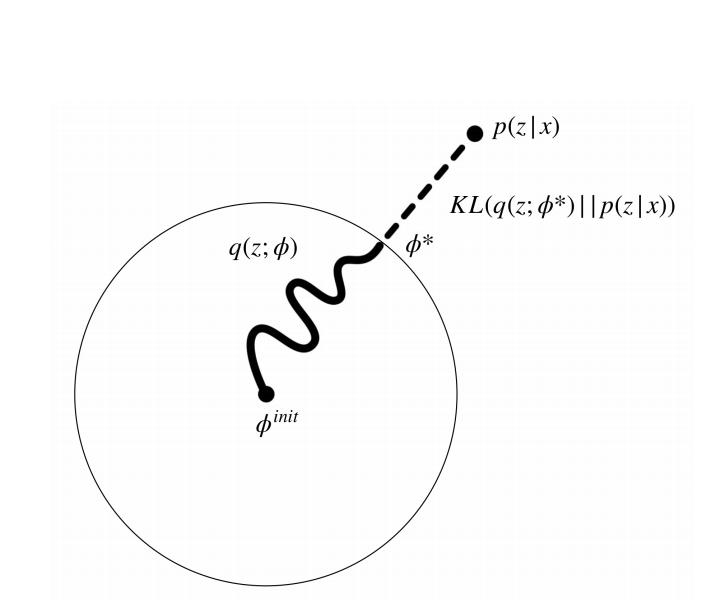
\includegraphics[scale=0.65]{elbo}
	\end{figure}
	
	
}





\frame[<+->]{
\frametitle{KL divergence}
\begin{itemize}

\item We measure the closeness of two distributions with Kullback-Leibler (KL) divergence.
\item We focus KL variational inference \citep{Blei+2016:VI}, where the KL divergence between $q(z)$ and $p(z|x)$ is optimised.
\begin{equation}
\begin{aligned}
\mathrm{KL}(q \| p)=\mathrm{E}_{q}\left[\log \frac{q(z)}{p(z | x)}\right]
\end{aligned}
\end{equation}
\item We can not minimize the KL divergence exactly, but we can maximise  a lower bound on the marginal likelihood.
\end{itemize}
	
	
}


\frame[<+->]{
\frametitle{Evidence lower bound}
\small{
\begin{itemize}

\item If we use the Jensen’s inequality applied to probability distributions. When $f$ is concave, \\
	$f(\mathrm{E}[X]) \geq \mathrm{E}[f(X)]$
\item We use Jensen’s inequality on the log probability of the observations\\
This is the evidence lower bound  (ELBO):
\begin{equation}
\begin{aligned}
 \log p_{\theta}(x) &=\log \int p_{\theta}(x | z) p_{\theta}(z) \mathrm{d} z \\ &=\log \int \frac{q_{\phi}(z)}{q_{\phi}(z)} p_{\theta}(x | z) p_{\theta}(z) \mathrm{d} z \\ 
 &=\log \mathbb{E}_{q}\left[\frac{p_{\theta}(x | z) p_{\theta}(z)}{q_{\phi}(z)}\right] \\ 
 & \geq \mathbb{E}_{q }\left[\log \frac{p_{\theta}(x | z) p_{\theta}(z)}{q_{\phi}(z)}\right] \\ 
 & =\mathbb{E}_{q }\left[\log \frac{p_{\theta}(z)}{q_{\phi}(z)}\right]+\mathbb{E}_{q }\left[\log p_{\theta}(x | z)\right] \\
 &=-\operatorname{KL}\left(q_{\phi}(z) \| p_{\theta}(z)\right)+\mathbb{E}_{q }\left[\log p_{\theta}(x | z)\right] \\ &=\mathcal{L}(\theta, \phi | x) 
\end{aligned}
\end{equation}

\end{itemize}
}
	
}

\frame{
\frametitle{ELBO}
\begin{itemize}
\item The objective  is to do optimization of the function $q_\phi(z)$ to maximize the ELBO:
\begin{equation}
\begin{aligned} \mathrm{KL}\left(q_{\phi}(z) \| p_{\theta}(z | x)\right) &=\mathbb{E}_{q }\left[\log \frac{q_{\phi}(z)}{p_{\theta}(z | x)}\right] \\ &=\mathbb{E}_{q }\left[\log q_{\phi}(z)-\log p_{\theta}(z | x)\right] \\ &=\mathbb{E}_{q }\left[\log q_{\phi}(z)-\log \frac{p_{\theta}(x | z) p_{\theta}(z)}{p_{\theta}(x)}\right] \\ &=\mathbb{E}_{q }\left[\log \frac{q_{\phi}(z)}{p_{\theta}(z)}\right]-\mathbb{E}_{q z}\left[\log p_{\theta}(x | z)\right]+\log p_{\theta}(x) \\ &=-\mathcal{L}(\theta, \phi | x)+\log p_{\theta}(x) \end{aligned}
\end{equation}
\end{itemize}
}


\frame[<+->]{
\frametitle{Evidence lower bound}
\begin{itemize}

\item To denote a lower bound on the log marginal likelihood:
\begin{equation}
	\begin{aligned} 
	\log p_{\theta}(\mathbf{x}) & \geq \log p_{\theta}(\mathbf{x})-\operatorname{KL}\left(q_{\phi}(\mathbf{z} | \mathbf{x}) \| p_{\theta}(\mathbf{z} | \mathbf{x})\right) \\ &=\mathbb{E}_{q}\left[\log p_{\theta}(\mathbf{x} | \mathbf{z})\right]-\mathrm{KL}(q_{\phi}(\mathbf{z} | \mathbf{x}) \| p(\mathbf{z})) \end{aligned}
	\end{equation}
\item  It lower-bounds the marginal distribution of $x$
	
\end{itemize}
	
	
}


\frame[<+->]{
\frametitle{Mean Field}
\begin{itemize}

\item We assume that the variational family factorises:
\begin{equation}
\begin{aligned}
q\left(z_{0}, \ldots, z_{N}\right)=\prod_{i}^{N} q\left(z_{i}\right)
\end{aligned}
\end{equation}
\item This simplification make optimisation and inference with VI tractable
	
\end{itemize}
	
	
}


\section{DGM4NLP}

\frame{
	\frametitle{Document modelling}
	\begin{itemize}
	\item  Know what topics are being discussed on Twitter and by what distribution they occur.
	\begin{figure}
	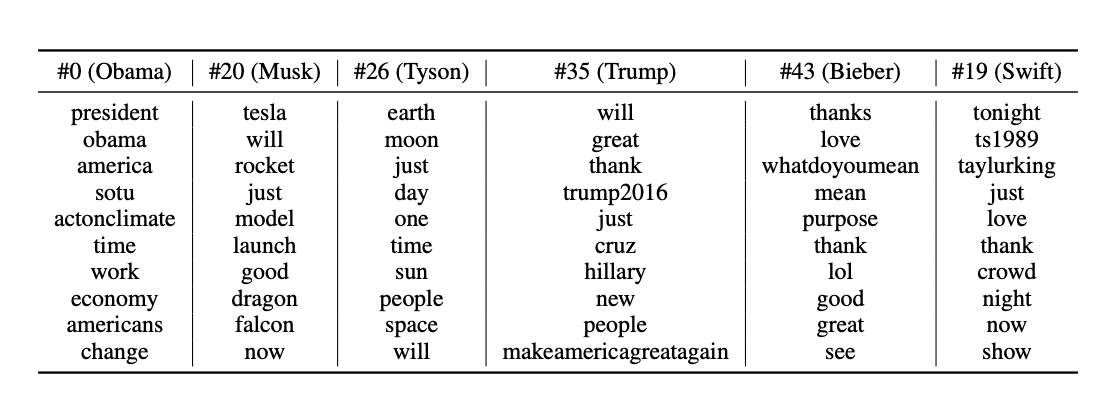
\includegraphics[scale=0.45]{topic_model}
	\end{figure}
	\end{itemize}

}

\frame{
	\frametitle{Word representation}
	
	\begin{figure}
	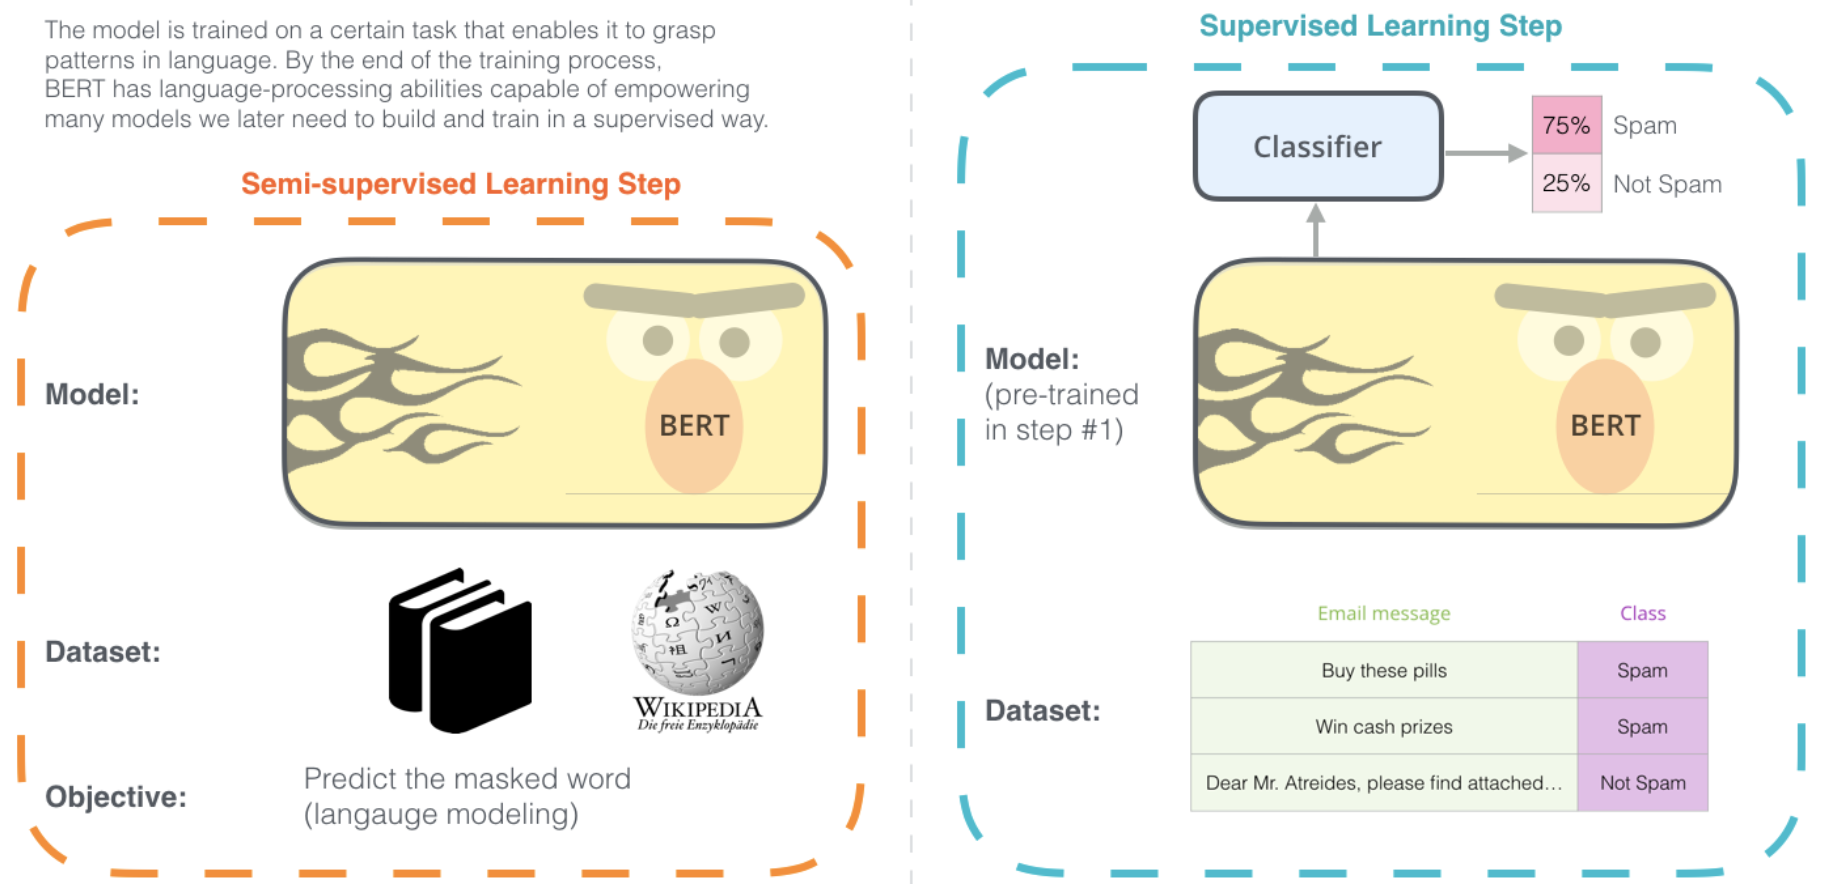
\includegraphics[scale=0.35]{bert}
	\end{figure}
	
}



\frame{
	\frametitle{Word representation}
	Generative model
	\begin{itemize}
	\item  Embed words as probability densities.
	\item Add extra information about the context.\\
	e.g. translations as a proxy to sense annotation.
	\begin{figure}
	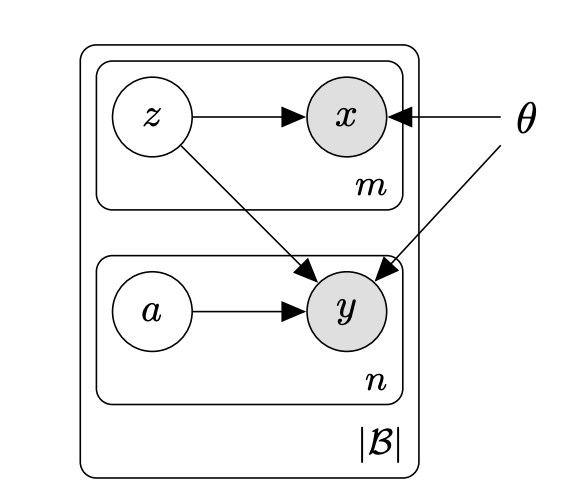
\includegraphics[scale=0.55]{embed_align}
	\end{figure}
	\end{itemize}
}



\frame[<+->]{
	\frametitle{Natural Language Inference}
	Classification
	\begin{itemize}
	\item 
	\begin{figure}
	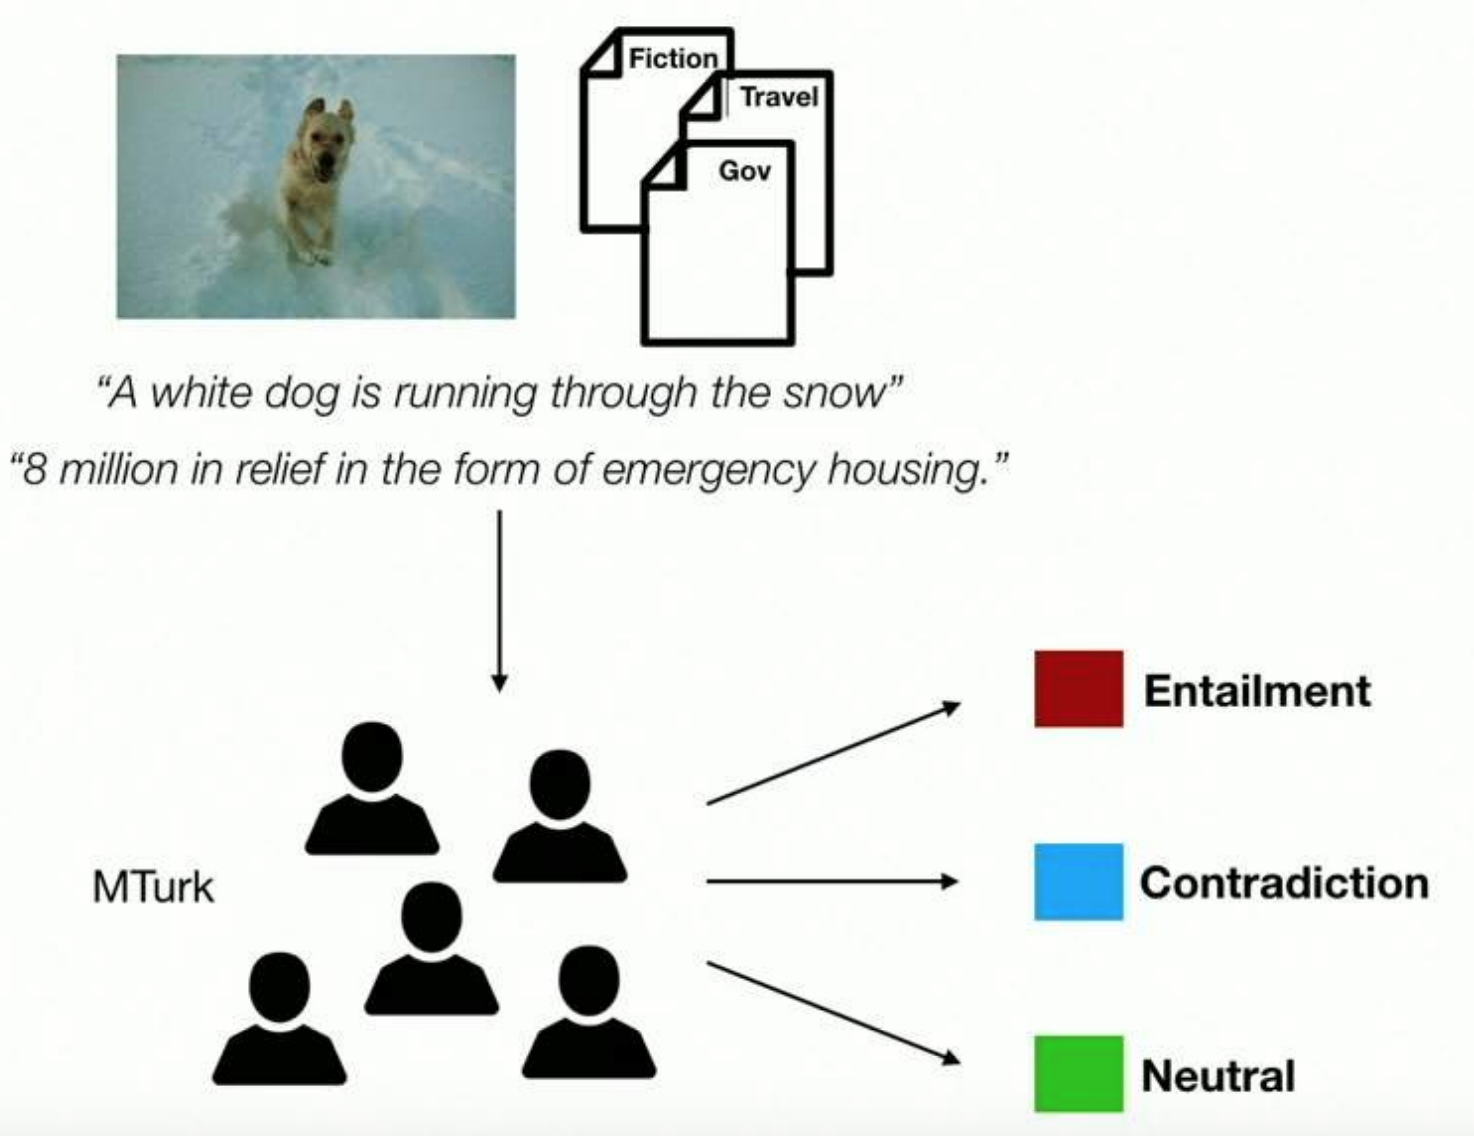
\includegraphics[scale=0.25]{nli_artifact2}
	\end{figure}
	\item 
	\begin{figure}
	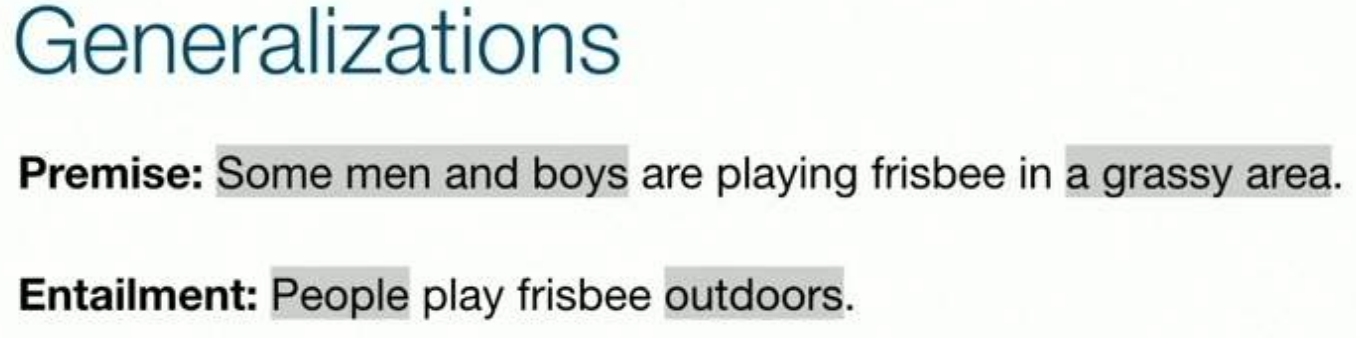
\includegraphics[scale=0.30]{nli_artifact3}
	\end{figure}
	\end{itemize}
	
	
}

\frame[<+->]{
	\frametitle{Natural Language Inference}
	Generative model
	\begin{itemize}
	\item Avoid over-fitting.
	\item Change of prior.
	\begin{figure}
	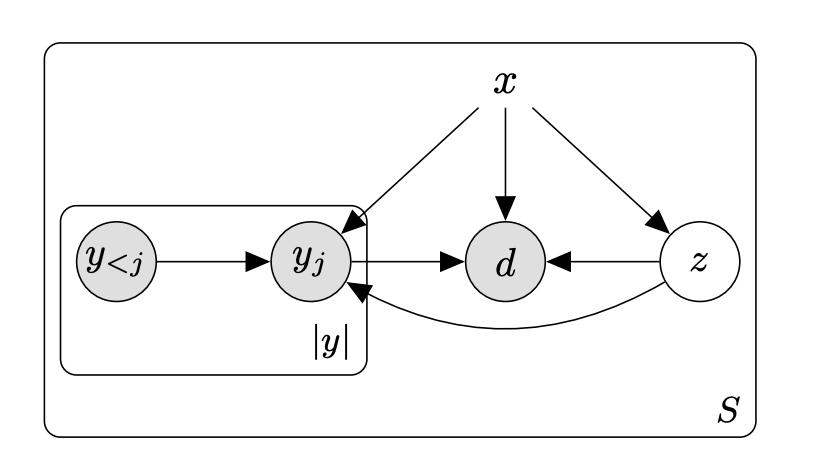
\includegraphics[scale=0.50]{nli_vae}
	\end{figure}
	\end{itemize}
	
	
}

\frame[<+->]{
	\frametitle{Natural Language Inference}
	Confidence of classification 
	\begin{itemize}
	\item  Bayesian NN
	\item  We place  a prior distribution over the model parameters $p(\theta)$
	\begin{figure}
	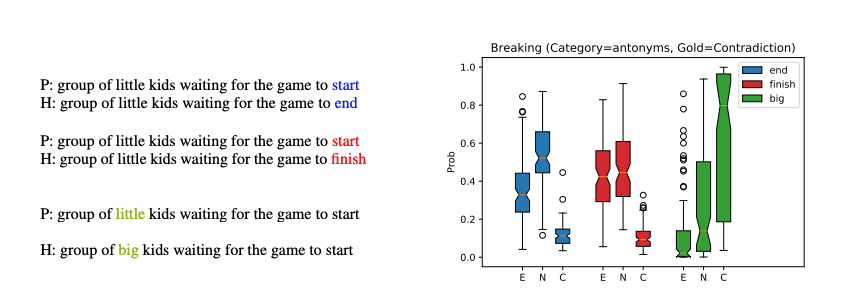
\includegraphics[scale=0.60]{mc}
	\end{figure}
	\end{itemize}
	
	
}

\frame[<+->]{
	\frametitle{Neural Machine Translation}
	\begin{itemize}
	\item 
	\begin{figure}
	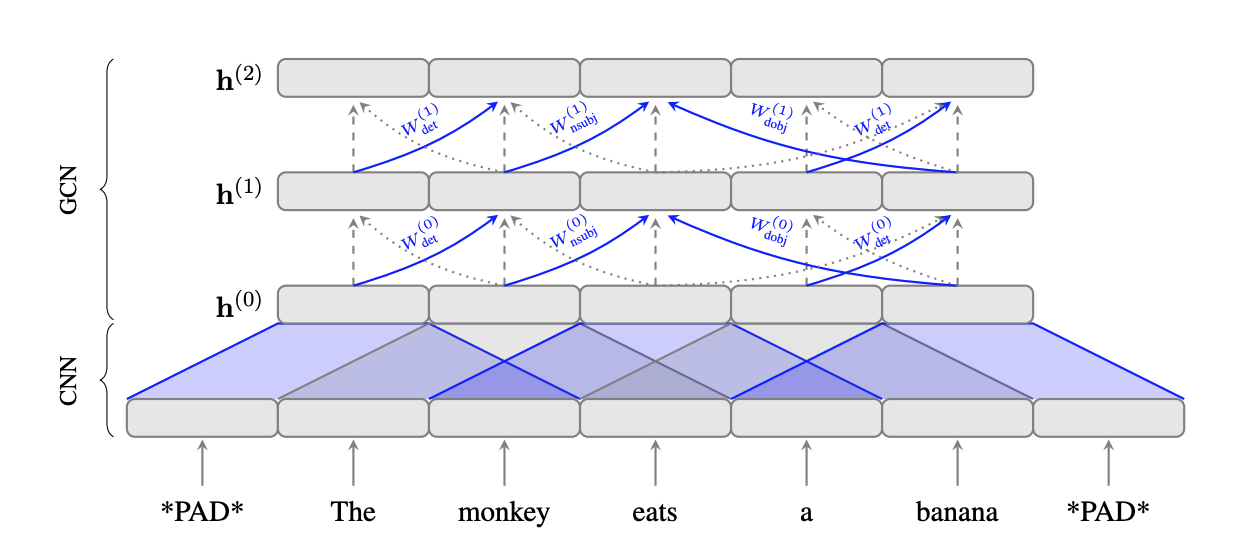
\includegraphics[scale=0.50]{gcn}
	\end{figure}
	\item 
	\begin{figure}
	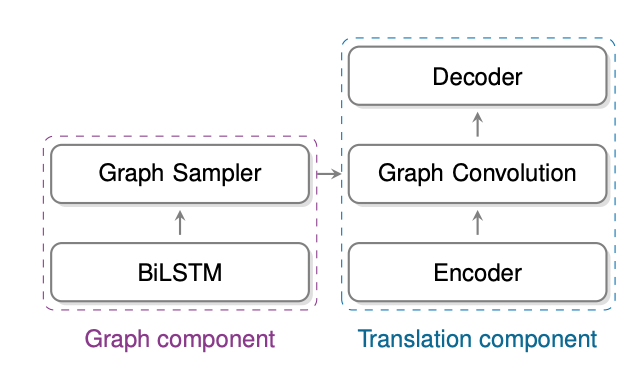
\includegraphics[scale=0.45]{gcn2}
	\end{figure}
	\end{itemize}
	
	
}


